
\appendix

\section{Appendix}
\subsection{Default units for Data Exchange entries}
\label{appendix:units}

The default units for Data Exchange entries follow the CXI entries definition, i.e. are SI based units (see table \ref{table:SI}) unless the "units" attribute is specified. Data Exchange prefers to use the default SI based units whenever possible.

\begin{table}[h!]\sffamily \small
\caption{SI (and common derived) base units for different quantities}
\label{table:SI}
\begin{center}
\centering
\rowcolors{1}{white}{tableBlue}
\begin{tabular}{p{4.5cm} p{4.5cm}  p{2.5cm}}
\doublerulesepcolor{tableBlue}
\toprule
\bfseries Quantity   & \bfseries Units & \bfseries Abbreviation \\
\doublerulesepcolor{tableBlue}
\midrule
length & meter & m \\
mass & kilogram & kg \\
time & second & s \\
electric current & ampere & A \\
temperature & kelvin & K \\
amount of substance & mole & mol \\
luminous intensity & candela & cd \\
\midrule
frequency & hertz & Hz \\
force & newton & N \\
pressure & pascal & Pa \\
energy & joule & J \\
power & watt & W \\
electric potential & volt & V \\
capacitance & farad & F \\
electric resistance & ohm & $\Omega$ \\
absorbed dose & gray & Gy \\
area & square meter & m\^{}2 \\
volume & cubic meter & m\^{}3 \\
\bottomrule
\end{tabular}
\end{center}
\end{table}


\subsubsection{Exceptions}
Angles are always defined in degrees {\em not} in radians and use the abbreviation "degree".

\subsubsection{Times and Dates} 
Times and Dates are always specified according to the \href{http://www.w3.org/TR/NOTE-datetime}{ISO 8601}.  This means for example ``1996-07-31T21:15:22+0600''. Note the ``T'' separating the data from the time and the ``+0600'' timezone specification.

\clearpage
\subsection{Geometry}
\subsubsection{Coordinate System}

The Data Exchange uses the same CXI coordinate system. This is a right handed system with the z axis parallel to the X-ray beam, with the positive z direction pointing away from the light source, in the downstream direction. The y axis is vertical with the positive direction pointing up, while the x axis is horizontal completing the right handed system (see Fig. \ref{fig:CoordSystem}). The origin of the coordinate system is defined by the point where the X-ray beam meets the sample.

\begin{figure}[h!]
\centering
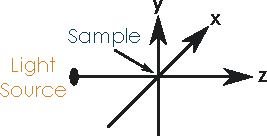
\includegraphics[width=0.6\textwidth]{figures/dx_CoordSystem.pdf}
\caption{The coordinate system used by CXI. The intersection of the X-ray beam with the sample define the  origin of the system. The z axis is parallel to the beam and points downstream.}
\label{fig:CoordSystem}
\end{figure}

\subsubsection{The local coordinate system of objects}
\label{OriginOfObjects}

For many detectors their location and orientation is crucial to interpret results.  Translations and rotations are used to define the absolute position of each object. But to be able to apply these transformations we need to know what is the origin of the local coordinate system of each object. Unless otherwise specified the origin should be assumed to be the geometrical center of the object in question. The default orientation of the object should have the longest axis of the object aligned with the x axis, the second longest with the y axis and the shortest with the z axis.

